\documentclass[12pt]{article}
%%%%%%%%%%%%%%%%%
% Imported Packages
%%%%%%%%%%%%%%%%%
\usepackage{setspace}
\usepackage{url}
\usepackage{multicol}
\usepackage{etoolbox}
\usepackage{relsize}
\patchcmd{\thebibliography}
  {\list}
  {\begin{multicols}{2}\smaller\list}
  {}
  {}
\appto{\endthebibliography}{\end{multicols}}

\usepackage{titlesec}
\usepackage{flushend}
\expandafter\def\expandafter\UrlBreaks\expandafter{\UrlBreaks%  save the current one
  \do\\\do-}

\usepackage{soul}

\usepackage{graphicx}
\graphicspath{ {images/} }

\usepackage{capt-of}

%%% PAGE DIMENSIONS
\usepackage[margin=1in]{geometry}
\geometry{letterpaper}

\begin{document}


%%%%%%%%%%%%%%%
% Title
%%%%%%%%%%%%%%%
\title{\vfill LiteCrypto} %\vfill gives us the black space at the top of the page
\author{
Team AES - Andrew Wang, Sam (Jiewen) Wu, and Elton Yang \vspace{10pt} \\
CPE 458: Current Topics in Computer Systems (Cryptographic Engineering)  \vspace{10pt} \\
Dr. Zachary Peterson \vspace{10pt} \\
}
\date{December 12, 2014} %Or use \today for today's Date

\maketitle

\vfill  %in combination with \newpage this forces the abstract to the bottom of the page
\begin{abstract}
\end{abstract}
\thispagestyle{empty} %remove page number from title page, but still keep it as pg #1
\newpage
\thispagestyle{empty}
\tableofcontents
\thispagestyle{empty}
\mbox{}
\newpage

%%%%%%%%%%%%%%%%%%%%
%%% Known Facts  %%%
%%%%%%%%%%%%%%%%%%%%
\begin{multicols}{2}
\section{Introduction}
\subsection{CubeSat}
CubeSat is a international collaborative project of over 40 educational systems and private firms. A CubeSat is a satellite that is 10 $cm^{3}$ and with a mass of 1.33 kg. \cite{CubeSat}
\subsection{PolySat}
PolySat is Cal Poly’s branch of CubeSat, and was established since 1999. Dr. Bellardo is the current advisor for PolySat. They have eight launched missions and three are currently in development. \cite{PolySat}
\section{Motivation and Background}
Our group decided on creating a CubeSat Crypto Library for our Crypto Engineering Final Project. 
\subsection{Background}
Dr. Bellardo has discussed with our team that the future of CubeSat is to allow them to move in space. However, their current communications from home base to the satellite is encrypted and unauthorized.  Therefore, an adversary who wishes to harm the CubeSat, or harm another object using the CubeSat, may sniff a command packet to the satellite and control it. Dr. Bellardo has given us a set of requirements that the library should have.
\subsection{Requirements}
\subsubsection{Binary Size}
Due to the small size of the CubeSat and the large amount of things it does, there is not a lot of storage space for the library. Therefore, the binary size needed to be around 50 kilobytes. Because the library would be part of its main functions, it will also need to be small for a quick boot time for the operating system. 
\subsubsection{Data Transfer}
Our library can not use transfer large amount of data between home base and the satellite. AX.25 speed limits on data are rarely higher than 9,600 bits/s and are usually 1,200 bits/s. \cite{AX25} The satellite also does not return an acknowledgement packet after successful retrieving a packet. Therefore, we are restricted on which scheme to use for our crypto library. Another issue is the connection time with the CubeSat is at most 15 minutes an hour due to the satellite orbiting the Earth. Therefore, we cannot use schemes that require a constant connection with the satellite. 
\subsubsection{Encryption and Authentication}
Our library should allow any user to have the option to encrypt or authenticate their packets. It should have 3 functions: No security, one way authentication, and authenticated encryption. Using the diagram on the next page is how Dr. Bellardo described how we should encrypt and authenticate. We were told to only encrypt the data portion of the packet, and only authenticate the IPv4 and UDP headers along with the data.
\begingroup
    \centering
    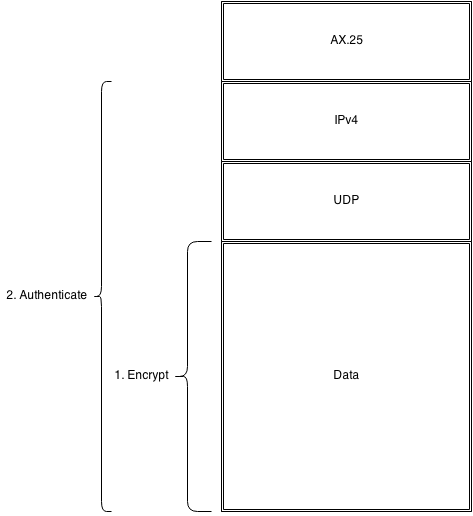
\includegraphics[width=7cm]{researchDiagram.png}
\endgroup
\section{Related Work/Research}
We began our research by looking for current satellite encryption. We found a paper on AES (Advanced Encryption Standard) with LDPC (Low Density Parity Check Code) in order to design a secure and reliable error correction method. \cite{SEEC} We also found that stream ciphers lead to serious problems if used incorrectly for satellite applications. \cite{stream_problems} We discovered someone else's work to authenticate IP protocol. \cite{IP_Protocol} In order to meet the low overhead requirement we found a low cost one-way HMAC proposal for a RFID system. \cite{HMAC_RFID} With all of this information, we needed a light weight software library for encryption to use. 
\subsection{CyaSSL (wolfSSL)}
CyaSSL is a lightweight SSL/TLS library. It advertised a special build called LeanPSK, which was an implementation of CyaSSL that could be built in as little as 20 kilobytes. LeanPSK is also 20 times smaller than OpenSSL, and uses 1 to 36 kilobytes of memory. This configuration required pre-shared keys. \cite{CyaSSL} However, after creating the binary ourselves and using their library, we found it to be complicated to build and the binary ended up to be 57 kilobytes. That was above our binary size requirement so we looked for a different library to use. 
\subsection{NaCl}
The NaCl crypto library has all of the core operations needed to build our crypto library. NaCl advertises state of the art security, improves usability, and improved speed. However the full NaCl library is too large for us to use, so we found a smaller version of the NaCl library to use. \cite{NaCl}
\subsubsection{TweetNaCl}
TweetNaCl supports 25 of the C NaCl functions used by applications and fits into a 100 tweets. It is self contained library so it was easy to build. \cite{TweetNaClPaper} However, it did not have HMAC build into TweetNaCl so we ported it from the original NaCl library. 

\section{Our Work}
\subsection{Key Exchange}

The LiteCrypto library revolves around symmetric key cryptography. The keys used for authentication and encryption in the LiteCrypto library are pre-shared (or secret) keys. The library expects a key to be provided for all cryptographic functions. In the context of the CubeSat, encryption and authentication keys need to be agreed upon before sending the device for launch into space. Since the LiteCrypto library only provides for cryptographic functions for satellite communications via AX.25/IPv4, the security of the keys in memory or disk used for the library is considered outside the realm of this project. Therefore, we assume the keys used for this library is appropriately secured by another system.

\subsubsection{Tradeoffs Made}

We decided not to perform public-key cryptography because we believed it would have been too much overhead for the CubeSat. The amount of data to be inserted into the packets would have been increased. However, TweetNaCl offers public-key cryptographic functions \cite{TweetNaClPaper}, so it is possible to easily implement public-key cryptography in LiteCrypto.

\subsection{Authentication}

Authentication in LiteCrypto utilizes NaCl library's HMAC-SHA512-256 authentication function. \footnote{TweetNaCl did not provide the function, so we ported the function from the full NaCl library over into the TweetNaCl source files for our use.} The HMAC-SHA512-256 authentication scheme essentially performs HMAC-SHA512 and truncates to the first 256 bits \cite{NaClSiteAuth}. This scheme is conjectured to meet the standard notion of unforgeability \cite{NaClSiteAuth}.

The sign function takes in a 32-byte key \cite{NaClSiteAuth} and variable-length IPv4 packet to output a signed IPv4 packet which has a 32-byte tag \cite{NaClSiteAuth} inserted in the head of the data portion. \footnote{Because we did get to perform live testing, we are unsure if this insertion breaks the IPv4 system. An alternative process for inserting the tag is possible.} The verify function takes a signed IPv4 packet and removes the inserted tag from the head of the data portion. Verification is then performed on the reconstructed packet by generating a new tag to compare with the provided tag. Based on the source files, the comparison in TweetNaCl is done by a constant-time string comparison function to avoid creating side-channels. If the packet verifies, the function outputs the new size of the reconstructed packet. Otherwise, it outputs -1 as ⊥.

\subsubsection{Tradeoffs Made}

We chose HMAC-SHA512-256 over TweetNaCl's one-time authentication because we wanted to be able to reuse the keys. With one-time authentication scheme, reusing a key to authenticate more than one message reveals enough information to allow for forgeries \cite{NaClSiteOneTimeAuth}.

\subsection{Encryption}

LiteCrypto utilizes TweetNaCl's secret-key encryption scheme based on xsalsa20 for encryption. The xsalsa20 scheme expands the amount of nonce bytes available to use for salsa20 \cite{TweetNaClPaper}. Because xsalsa20 uses salsa20 as the core, the security of xsalsa20 depends on the security of the salsa20 scheme \cite{TweetNaClPaper}. The xsalsa20 encryption scheme is conjectured to meet the standard notion of unpredictability \cite{NaClSiteStream}.

The TweetNaCl encryption function generates a key stream from xsalsa20 using a 32-byte key and a 24-byte nonce \cite{NaClSiteStream}, so it effectively acts as a stream cipher \cite{TweetNaClPaper}. The key stream is deterministic in that the same key and nonce pair will generating the same key stream. The key stream is bitwise XORed with the plaintext to produce the ciphertext \cite{TweetNaClPaper}. Note that the encryption scheme does not hide the length of the message \cite{NaClSiteStream}. Because the function acts as a stream cipher, the function can be used both to encrypt or decrypt. We base our encryption function around the use of TweetNaCl's function.

The encrypt function takes in a 32-byte key \cite{TweetNaClPaper} and a variable-length IPv4 packet to output a IPv4 packet with 24-byte nonce inserted at the head of the encrypted data. The IPv4 packet headers are left untouched in plaintext. The nonce is randomly generated by the function by reading from urandom. The NaCl group supports that the “nonces are long enough that randomly generated nonces have negligible risk of collision.” \cite{NaClSiteStream} The size of the encrypted packet is returned on success; otherwise, -1 is returned.

The decrypt function takes in a 32-byte key \cite{TweetNaClPaper} and a variable-length encrypted IPv4 packet to output a decrypted IPv4 packet with the nonce bytes removed. The nonce bytes are removed from the head of the encrypted data of the given encrypted packet. The encrypted data is then decrypted using the provided key and nonce bytes. We construct the new packet by appending the decrypted data to the IPv4 headers. The size of the decrypted packet is returned on success; otherwise, -1 is returned.

\subsection{Authenticated Encryption}

Authenticated encryption in LiteCrypto makes use of the authentication and encryption functions discussed above. To encrypt a packet, we first perform our encryption scheme then our authentication scheme. We have ultimately inserted 56 bytes into the IPv4 packet: 32 bytes from authentication tag and 24 bytes from encryption nonce. To decrypt, we first attempt to verify the packet. If the packet verifies, we perform our decryption scheme and output the decrypted packet without the 56 bytes originally inserted; otherwise, -1 is outputted as ⊥. Our encrypt-sign and verify-decrypt schemes achieve authenticated encryption by never decrypting a non-authenticated packet.

Because we have intermediate states between encrypt-sign and verify-decrypt, we have dynamically allocated memory to contain the intermediate states. On memory allocation error, the function returns -1. Having the dynamically allocated memory does not decrease the security of LiteCrypto since the intermediate states only contain the IPv4 header which is left in plaintext at all times, the nonce bytes, and the encrypted data. An adversary would not gain any more information than if he or she caught an encrypted packet.

\subsection{PBKDF2}

The keys used for authentication and encryption in LiteCrypto are expected to be 32 bytes long. For the users' convenience, we have included a specialized password-based key-derivation function for this library. The function takes in two user provided parameters: a variable-length key and a 16-byte salt. The function outputs a 32-byte key to the specified location and returns the size of the key on success. On failure, the key-derivation function returns -1.

The key-derivation scheme follows the standard PBKDF2 scheme from \cite{PBKDF2Standard} with SHA512 as the underlying pseudo-random function. Since SHA512's digest size is 64 bytes \cite{NaClSiteHash} and our required key size is only 32 bytes, we only have one block under the PBKDF2 scheme. Because we always have only one block, we have omitted the block number from the initial iteration in evaluating U1 of the block. Excluding U1 which uses the user-provided salt, we perform ten thousand iterations with each iteration using the previous iteration's output as salt on the user-provided key \cite{PBKDF2Standard}. All iterations are then bitwise XORed together to form the output key \cite{PBKDF2Standard}.

\section{Evaluation and Analysis}
\subsection{Performance}
Because performance is dependent on instruction optimization, the most efficient programs are compiled specifically for a certain processor architecture. In order to reduce space, tweetNaCl cannot provide optimal run-time performance. \cite{TweetNaCl} While tweetNaCl is not fully optimized for the processor, the impact on a low-volume cryptographic communication like the CubeSat is minimal.
\subsubsection{-Os vs -O2 Optimization Flag}
Most typical applications use the -O2 flags for improved performance, but on a space limited platform, the -Os flag is more useful. The -Os flag enables all -O2 flags that typically do not increase size as well as performing more optimizations to reduce size. \cite{GCCOP} 
\subsection{Testing}
In order to ensure the functionality of the library, we tested generated our own test cases. We were able to verify, encrypt, and decrypt messages successfully. Due to a lack of proper hardware, the program was not tested live on a CubeSat and with actual packets. The other option besides testing directly on a CubeSat would be to test it against a CubeSat virtual machine, but the communications for the CubeSat require additional libraries that we were not provided. In this situation, we would provide the library to the CubeSat team and have them perform functionality tests according to their needs.
\subsection{Future Work}
While the initial library is completed, there are many features that can be added with minimal impact to the size constraints.
\subsubsection{Key Exchange by PKE}
If a key pair needs to be updated for some reason, we currently require direct access to the CubeSat in order to replace and verify the key. Because we currently use only the initial key pair, if the key was compromised, the CubeSat would be vulnerable to a user with malicious intent. In order to mitigate such risks, a key exchange algorithm should be implemented to allow the update of keys used for communication.
\subsubsection{Forward Secrecy}
Forward Secrecy would allow for past communications to stay private even when an attack is successful in compromising the private key. Because all the past communications were protected by forward secrecy, the attacker would not be able to decrypt previous messages. This is crucial if the CubeSat is communication confidential information.
\subsubsection{Sequence Numbers}
This would prevent replay attacks. Because communication to the Cubesat is not stable, packets are resent continuously while the cubesat is in range. This increases the chance that the Cubesat has received the packet. With unstable communication, if the Cubesat did receive the packet, a response packet may not be received by the sender. This form of communication means that the process of repeating the message to the Cubesat can cause a replay attack by an official source. While replaying a command may not affect the mission, there is concern when it is crucial for the Cubesat to receive the command only once. Such commands include movement, a concept that may be implemented in Cubesats in the future. If movement is implemented in the Cubesat, the Cubesat cannot be allowed to replay a movement otherwise there is the possibility the Cubesat can be knocked out of orbit or into another satellite. The simplest way to mitigate this risk is through sequence numbers. Because the official source would issue out one sequence number per command, a repeated packet would not affect the Cubesat once it parses the packet. As long as encryption remains secure, there is no concern over another entity forging a sequence number. This leads to the last case, a used sequence number with a different command. The only time this would happen through non-malicious means is if sequence number exceeds the amount of numbers allowed. In this situation, there should be some sort of authentication to alert the Cubesat that the sequence number should be reset. In the case of a sequence reset, measures should be taken so that an attacker collecting old packets cannot then send them to the Cubesat in attempts to get the Cubesat to perform a task.
\section{Conclusion}
\end{multicols}
\clearpage
%cite all the references from the bibtex you haven't explicitly cited
\nocite{*}
%break long urls with lots of hyphens
\def\UrlBreaks{\do\/\do-}

\bibliographystyle{IEEEannot}

\bibliography{paper}
\end{document}